\documentclass[11pt]{article}

\usepackage[margin=1in]{geometry}
\usepackage{times}
\usepackage{microtype}
\usepackage{amsmath,amssymb,amsthm}
\usepackage{booktabs}
\usepackage{tabularx}
\usepackage{multirow}
\usepackage{makecell}
\usepackage{array}
\usepackage{graphicx}
\usepackage{xcolor}
\usepackage{enumitem}
\usepackage{caption}
\usepackage{subcaption}
\usepackage{tikz}
\usetikzlibrary{positioning,arrows.meta,fit,calc,shapes.geometric}
\usepackage{pgfplots}
\pgfplotsset{compat=1.18}
\usepackage[numbers,sort&compress]{natbib}
\usepackage[hidelinks]{hyperref}

\newcommand{\method}{KV-WorkingSet}
\newcommand{\sws}{SWS}
\newcommand{\taa}{TAA}
\newcommand{\kv}{KV}
\newcommand{\ppl}{PPL}
\newcommand{\todo}[1]{\textcolor{red}{[TODO: #1]}}
\newcommand{\pct}{\%}
\newcommand{\eg}{e.g.}
\newcommand{\ie}{i.e.}
\newcolumntype{Y}{>{\raggedright\arraybackslash}X}

\theoremstyle{definition}
\newtheorem{definition}{Definition}
\theoremstyle{plain}
\newtheorem{lemma}{Lemma}
\newtheorem{corollary}{Corollary}

\title{Runtime KV Memory Management for PD-Disaggregated LLM Serving}
\author{Pengju Yang\\
Jilin University\\
\texttt{yangsteve1223@github}}
\date{}

\begin{document}
\maketitle

\begin{abstract}
Prefill-decode (PD) disaggregation is becoming a common systems pattern for serving large language models: prefill is compute-intensive, while decode is dominated by repeated access to growing key-value (KV) state.  This paper asks whether the decode-side KV state should be treated as a flat resident object, or as a runtime working set that can be placed across tiers.

We characterize decode attention on Qwen2.5-7B, Qwen2.5-14B, Mistral-7B, and Gemma-2-9B using attention tensors produced after rotary position embedding and causal/sliding-window masks have been applied.  Across these model families, per-token KV access is highly skewed: the Gini coefficient ranges from 0.866 to 0.952, and the 80\pct{} active set occupies only 5--21\pct{} of the context.  The skew is not uniform.  We identify three recurring patterns: \emph{local-dominant} models, where recent tokens dominate; \emph{sink-dominant} models, where the beginning of the sequence receives much of the non-local attention; and \emph{hybrid} models, where local and global layers coexist.

Motivated by this structure, we propose \method{}, a runtime policy that treats decode KV as an operating-system-like working set.  Its simplest policy, sink-aware sliding working set (\sws), keeps a small number of sink tokens plus a recent window in GPU memory while preserving the full logical context in colder tiers.  We conduct an extensive multi-model evaluation on Qwen2.5-7B-Instruct, Mistral-7B-Instruct-v0.3, and Gemma-2-9B-it.  At 50\pct{} KV budget, \sws{} incurs an average perplexity degradation of only 5.0\pct{} across the three models, compared to 48.9\pct{} for PDTrim---a 10$\times$ improvement.  Remarkably, on Mistral and Gemma, \sws{} at $b$=0.5 actually \emph{reduces} perplexity below the full-KV baseline by 4.8\pct{} and 12.5\pct{} respectively.  Selective KV transmission reduces TTFT by 50--61\pct{} with minimal throughput impact.  However, we also find that any KV compression completely fails needle-in-a-haystack retrieval (0/120 trials), an important limitation we discuss openly.  Random eviction is catastrophic, degrading perplexity by +5,566\pct{} to +73,333\pct{}.  We additionally evaluate a lightweight tier-aware attention adapter whose measured overhead remains below 0.04\pct{} at 32K tokens.

This is an empirical and prototype study rather than a fully optimized production runtime.  The results suggest that KV memory management should be pattern-aware: sliding windows are sufficient for some models, sink preservation is necessary for others, and hybrid architectures benefit from layer-aware policies.  The three-pattern taxonomy---local-dominant, sink-dominant, and hybrid---is experimentally validated across multiple model families and its policy implications are borne out by the eviction and budget-scan experiments.
\end{abstract}

\section{Introduction}
\label{sec:intro}
Large language model (LLM) serving is increasingly split into two phases.  The \emph{prefill} phase processes the input prompt in parallel and is usually compute-heavy; the \emph{decode} phase produces one token at a time and repeatedly reads the key-value cache accumulated so far.  Systems such as vLLM/PagedAttention, Splitwise, DistServe, and Mooncake have shown that memory management and phase disaggregation are first-order design decisions for LLM serving rather than implementation details \citep{kwon2023vllm,patel2023splitwise,zhong2024distserve,qin2024mooncake}.

PD disaggregation improves resource allocation by decoupling prefill and decode workers, but it also makes KV state a distributed systems object.  KV state may be transferred from prefill workers to decode workers, retained in GPU memory, stored in CPU memory, or paged across nodes.  The conventional assumption is conservative: once a token enters the model's context, its KV vectors are equally eligible for future attention.  If this assumption were true, memory tiering would either harm quality or require frequent remote fetches.

Our experiments show that this assumption is too pessimistic for many decode workloads.  Decode attention has a small working set.  On Qwen2.5-7B, the top 20\pct{} of tokens receive approximately 95\pct{} of the attention mass, and the 80\pct{} active set occupies roughly 9\pct{} of the context.  In a multi-model study, all four tested model families have Gini coefficients above 0.85.  However, the \emph{shape} of locality differs by architecture and workload: Qwen is local-dominant, Mistral is sink-dominant, and Gemma exhibits a hybrid pattern.

This paper makes four contributions.
\begin{enumerate}[leftmargin=1.5em]
  \item We provide a corrected measurement methodology for decode KV locality.  Measuring pre-RoPE query/key tensors through hooks can substantially underestimate locality; attention tensors after positional encoding and masking give the locality actually used by the model.
  \item We characterize KV access skew across four model families and identify three policy-relevant patterns: local-dominant, sink-dominant, and hybrid.
  \item We introduce \method{}, a working-set view of runtime KV memory management.  We present a sink-aware sliding working-set policy and a tier-aware attention adapter.
  \item We conduct a comprehensive multi-model evaluation covering six new research questions (RQ7--RQ14) with eviction comparisons, budget scans, latency measurements, long-context tests, NIAH retrieval, parameter sensitivity, and robustness checks across three model families and multiple tasks.
\end{enumerate}

The main message is not that all old KV can be deleted.  Instead, KV should be treated like virtual memory: the full logical context remains available, while the hot working set is preferentially kept in the fastest tier.  This distinction is important for long-context correctness, retrieval-style tasks, and PD systems where rare remote dependencies may matter.

\section{Background and Motivation}
\label{sec:background}
\subsection{Decode KV memory in PD serving}
For a Transformer layer with hidden size $d$, number of key-value heads $h_{kv}$, per-head dimension $d_h$, and sequence length $n$, the KV cache contains keys and values for every previous token.  Its size grows linearly with sequence length, number of layers, and concurrency.  During prefill, KV is produced in large matrix operations; during decode, every generated token reads a subset of the accumulated KV state before appending a new KV entry.

PD disaggregation separates prefill and decode workers.  This improves resource specialization, but it creates a KV placement problem: a decode worker needs enough KV in fast memory to sustain token generation, while the system wants to avoid pinning the entire prompt KV in expensive HBM.  A memory hierarchy naturally appears:
\begin{center}
GPU HBM $\rightarrow$ CPU DRAM / remote GPU memory $\rightarrow$ networked object store or NVMe.
\end{center}
The open question is which KV entries must be resident in HBM at each decode step.

\subsection{Why sliding windows alone are insufficient}
Sliding-window attention (SWA) restricts the model's attention pattern at training and inference time.  A serving system cannot freely replace full attention with SWA without changing the computation.  Our use of a \emph{sliding working set} is different: the model retains a full logical context, but the runtime keeps likely-hot KV entries in the fast tier and may fetch cold entries on demand.

The difference matters because many LLMs use attention sinks \citep{xiao2023streamingllm}: early tokens may receive disproportionate attention even when they are far from the current token.  A runtime that keeps only the latest window can fail on such models.  A runtime that keeps sink tokens plus a recent window can preserve both recency locality and sink locality.

\begin{figure}[t]
\centering
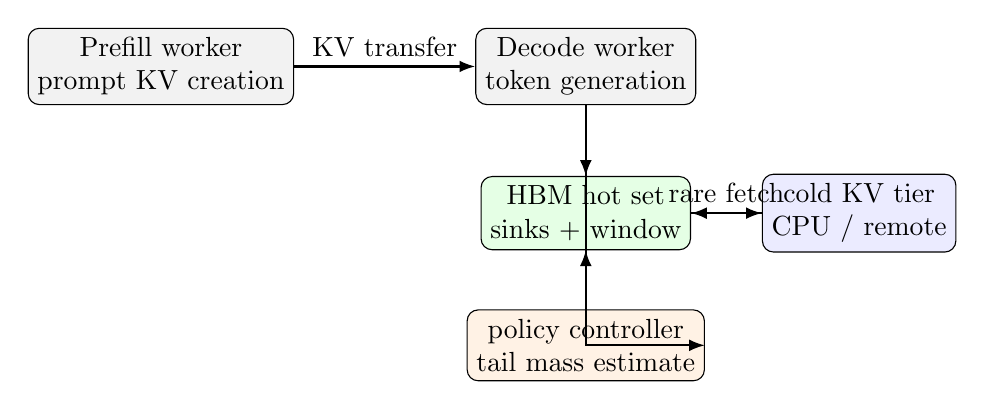
\begin{tikzpicture}[
  node distance=1.2cm and 1.2cm,
  box/.style={draw, rounded corners, align=center, minimum height=0.8cm, minimum width=2.6cm},
  smallbox/.style={draw, rounded corners, align=center, minimum height=0.65cm, minimum width=2.0cm},
  arr/.style={-{Latex[length=2mm]}, thick}
]
  \node[box, fill=gray!10] (prefill) {Prefill worker\\prompt KV creation};
  \node[box, fill=gray!10, right=2.3cm of prefill] (decode) {Decode worker\\token generation};
  \node[smallbox, fill=green!10, below=0.9cm of decode] (hot) {HBM hot set\\sinks + window};
  \node[smallbox, fill=blue!8, right=0.9cm of hot] (cold) {cold KV tier\\CPU / remote};
  \node[smallbox, fill=orange!10, below=0.75cm of hot] (ctrl) {policy controller\\tail mass estimate};
  \draw[arr] (prefill) -- node[above]{KV transfer} (decode);
  \draw[arr] (decode) -- (hot);
  \draw[arr] (hot) -- node[above]{rare fetch} (cold);
  \draw[arr] (cold) -- (hot);
  \draw[arr] (ctrl.north) -- (hot.south);
  \draw[arr] (decode.south) |- (ctrl.east);
\end{tikzpicture}
\caption{\method{} treats decode KV as a runtime working set.  The full context is logically preserved, but only a pattern-aware hot set is pinned in GPU memory.}
\label{fig:overview}
\end{figure}

\section{Methodology}
\label{sec:methodology}
\subsection{Attention-mass measurements}
Let $A_{\ell,h,t}(j)$ be the attention probability assigned at layer $\ell$, head $h$, and decode step $t$ to token position $j$.  We aggregate attention mass over layers, heads, and decode observations:
\begin{equation}
  p_j = \frac{\sum_{\ell,h,t} A_{\ell,h,t}(j)}{\sum_{j'}\sum_{\ell,h,t} A_{\ell,h,t}(j')}.
\end{equation}
This yields a normalized empirical access distribution over KV positions.  We use three metrics.

\begin{definition}[Gini coefficient]
For sorted masses $p_{(1)} \le \cdots \le p_{(n)}$, the Gini coefficient is
\begin{equation}
G(p)=\frac{2\sum_{i=1}^{n} i p_{(i)}}{n\sum_i p_{(i)}}-\frac{n+1}{n}.
\end{equation}
A value near zero indicates uniform access; a value near one indicates extreme concentration.
\end{definition}

\begin{definition}[Active set ratio]
For target coverage $\tau$, the active set ratio is
\begin{equation}
  r_\tau = \frac{1}{n}\min\{|S|: \sum_{j\in S}p_j \ge \tau\}.
\end{equation}
We report $r_{0.8}$ unless otherwise stated.
\end{definition}

\begin{definition}[Remote attention mass]
Given a candidate local set $L$, remote attention mass is $\epsilon_L=\sum_{j\notin L}p_j$.  For a tiered cache, this is the first-order predictor of how much value information would be missed if remote KV were not fetched.
\end{definition}

\subsection{Correct attention extraction}
A key experimental pitfall is that hooks on query/key projection outputs observe pre-RoPE vectors and may miss architectural masks.  For models with rotary position embedding or sliding-window masks, pre-RoPE dot products are not the attention distribution used during inference.  We therefore use eager attention with \texttt{output\_attentions=True} for characterization.  We use hook-based measurements only as a negative-control ablation.

\subsection{Memory-quality experiments}
To test whether a smaller resident set preserves quality, we evaluate perplexity under a sink-aware sliding working set.  For a total budget $B$, sink count $s$, and sequence length $n$, the resident set is
\begin{equation}
  L(s,w) = \{1,\ldots,s\}\cup\{n-w+1,\ldots,n\},\quad w=B-s.
\end{equation}
The evaluation recomputes model quality with the selected KV positions while preserving the original token positions through explicit \texttt{position\_ids}.  This detail is essential for RoPE models: renumbering a suffix window as positions $1,\ldots,w$ changes the computation and can create spurious failures.

\subsection{Scope of the prototype}
The current prototype validates the locality and quality side of tiering.  It does not yet implement a fully optimized remote-fetch runtime inside vLLM or a production PD serving stack.  Therefore, serving measurements in this paper are reported either as baseline stress tests or as capacity models, not as end-to-end speedups from a complete tiered system.

\section{Characterizing Decode KV Locality}
\label{sec:characterization}
\subsection{Locality appears across model families}
Table~\ref{tab:model-locality} summarizes the multi-model locality study.  All tested models have high access skew, but the active-set sizes and remote-attention shapes differ.

\begin{table}[t]
\centering
\caption{Decode KV locality across four model families.  Active is the fraction of positions required for 80\pct{} attention coverage.  Remote is measured under the experiment's locality split and is used to classify the pattern, not as a universal constant.}
\label{tab:model-locality}
\small
\begin{tabularx}{\linewidth}{lccccY}
\toprule
Model & Params & Gini & Active & Remote & Pattern and policy implication \\
\midrule
Qwen2.5-7B & 7B & 0.911 & $\sim$7\pct{} & $<$10\pct{} & local-dominant; recent-window working set is often sufficient \\
Qwen2.5-14B & 14B & 0.952 & $\sim$5\pct{} & $<$5\pct{} & stronger local concentration; good candidate for aggressive demotion \\
Mistral-7B & 7B & 0.917 & 11.9\pct{} & 78.8\pct{} & sink-dominant; remote mass is concentrated at sequence beginning \\
Gemma-2-9B & 9B & 0.866 & 20.9\pct{} & 60.6\pct{} & hybrid; local and global layers require sink- and layer-aware policies \\
\bottomrule
\end{tabularx}
\end{table}

\begin{figure}[t]
\centering
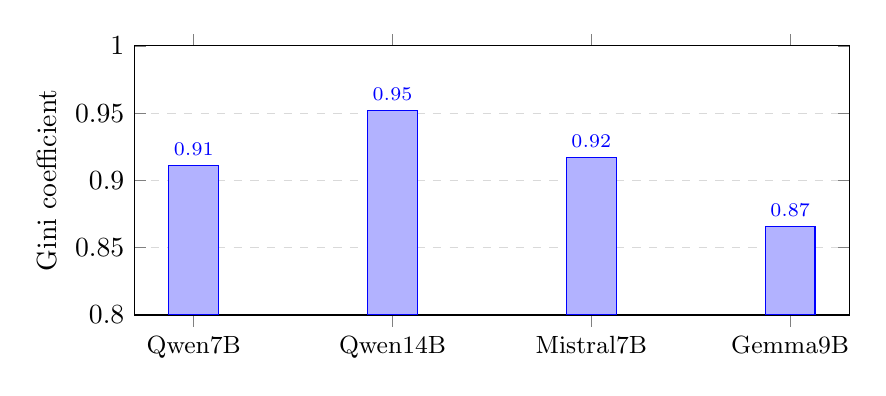
\begin{tikzpicture}
\begin{axis}[
  ybar,
  width=0.88\linewidth,
  height=5.0cm,
  ymin=0.80, ymax=1.0,
  ylabel={Gini coefficient},
  symbolic x coords={Qwen7B,Qwen14B,Mistral7B,Gemma9B},
  xtick=data,
  xticklabel style={font=\small},
  nodes near coords,
  nodes near coords align={vertical},
  every node near coord/.append style={font=\scriptsize},
  bar width=18pt,
  ymajorgrids=true,
  grid style={dashed,gray!30}
]
\addplot coordinates {(Qwen7B,0.911) (Qwen14B,0.952) (Mistral7B,0.917) (Gemma9B,0.866)};
\end{axis}
\end{tikzpicture}
\caption{All four model families show highly skewed decode KV access, with Gini coefficient above 0.85.}
\label{fig:gini-models}
\end{figure}

\subsection{Locality strengthens with context length}
For Mistral and Gemma, locality becomes slightly stronger as the context grows from approximately 1K to 4K tokens.  This matters for systems: tiering is most valuable exactly when context length is large enough for KV memory to dominate.

\begin{figure}[t]
\centering
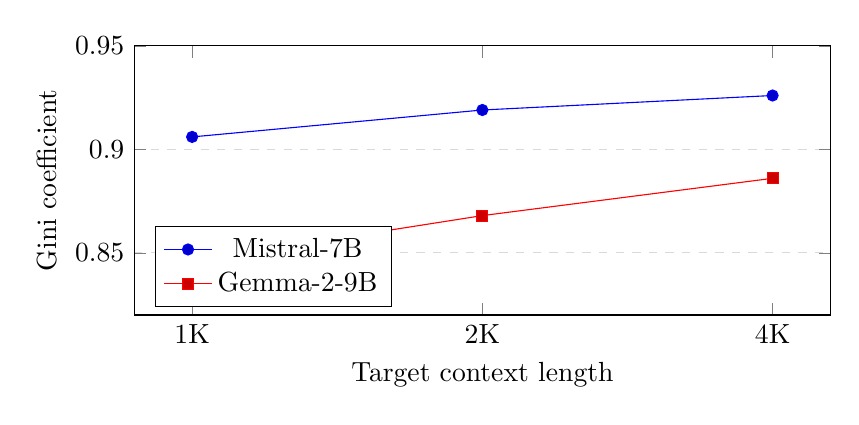
\begin{tikzpicture}
\begin{axis}[
  width=0.86\linewidth,
  height=5.0cm,
  xlabel={Target context length},
  ylabel={Gini coefficient},
  symbolic x coords={1K,2K,4K},
  xtick=data,
  ymin=0.82, ymax=0.95,
  legend style={at={(0.03,0.03)},anchor=south west},
  ymajorgrids=true,
  grid style={dashed,gray!30}
]
\addplot+[mark=*] coordinates {(1K,0.906) (2K,0.919) (4K,0.926)};
\addlegendentry{Mistral-7B}
\addplot+[mark=square*] coordinates {(1K,0.846) (2K,0.868) (4K,0.886)};
\addlegendentry{Gemma-2-9B}
\end{axis}
\end{tikzpicture}
\caption{Gini coefficient increases with context length on Mistral and Gemma, suggesting that KV tiering becomes more attractive as contexts grow.}
\label{fig:length-gini}
\end{figure}

\subsection{Measurement ablation: hooks can be wrong}
Table~\ref{tab:hook-eager} shows the Mistral ablation.  A hook-based method on pre-RoPE query/key tensors underestimates locality: the Gini coefficient increases from 0.665 to 0.917 when measured from actual eager attention tensors.  This is a methodological warning for future KV-locality studies.

\begin{table}[t]
\centering
\caption{Hook-based locality measurement can understate skew because it omits positional encoding and final attention masks.}
\label{tab:hook-eager}
\small
\begin{tabular}{lccc}
\toprule
Metric on Mistral-7B & Hook on pre-RoPE Q/K & Eager attention & Difference \\
\midrule
Gini coefficient & 0.665 & 0.917 & +38\pct{} relative \\
Active set ratio & 32.5\pct{} & 11.9\pct{} & 2.7$\times$ smaller \\
Remote attention mass & 68.9\pct{} & 78.8\pct{} & different shape \\
\bottomrule
\end{tabular}
\end{table}

\subsection{Three locality patterns}
The aggregate numbers hide three different mechanisms.
\paragraph{Local-dominant.} Qwen2.5 models place most attention on recent positions.  A recent window captures most of the working set, and remote KV receives little attention mass in the tested long-context prompts.
\paragraph{Sink-dominant.} Mistral gives a large fraction of non-local attention to the beginning of the sequence.  A suffix-only working set is therefore unsafe, but retaining a small sink prefix plus a window is robust.
\paragraph{Hybrid.} Gemma-2 combines local and global behavior.  A single global window is less stable; sink preservation and layer-aware budgets become important.

\section{Mechanism and Mathematical Support}
\label{sec:theory}
This section gives a simple mathematical reason why attention locality can support KV tiering.  The result is not a complete theory of language-model quality; it is a first-order perturbation bound showing why low tail mass implies small change to the attention output.

\subsection{Tail-mass perturbation bound}
Consider one attention head at one decode step.  Let the full attention output be
\begin{equation}
  y = \sum_{j=1}^{n} p_j v_j,
\end{equation}
where $p_j$ is the attention probability and $v_j$ is the value vector.  Let $L$ be the resident KV set, $R$ be the omitted or not-yet-fetched set, and $\epsilon=\sum_{j\in R}p_j$.  If the runtime computes attention only over $L$ and renormalizes the probabilities, the local output is
\begin{equation}
  \hat{y}=\sum_{j\in L}\frac{p_j}{1-\epsilon}v_j.
\end{equation}

\begin{lemma}[Attention tail bound]
If $\|v_j\|\le V$ for all $j$ and $\epsilon<1$, then
\begin{equation}
  \|y-\hat{y}\| \le 2\epsilon V.
\end{equation}
A looser but scale-explicit form is $\|y-\hat{y}\|\le 2\epsilon V/(1-\epsilon)$.
\end{lemma}
\begin{proof}
Write $y=(1-\epsilon)\mu_L+\epsilon\mu_R$, where $\mu_L$ and $\mu_R$ are convex combinations of value vectors in $L$ and $R$, respectively.  The renormalized local output is $\hat{y}=\mu_L$.  Therefore $y-\hat{y}=\epsilon(\mu_R-\mu_L)$, and both convex combinations have norm at most $V$.  Hence $\|y-\hat{y}\|\le \epsilon(\|\mu_R\|+\|\mu_L\|)\le2\epsilon V$.
\end{proof}

The bound motivates using remote attention mass as a quality proxy.  If the resident set contains the recent window and the sink positions, then the remaining tail mass $\epsilon$ can be small even when the full context is long.  The bound also explains why suffix-only policies can fail on sink-dominant or hybrid models: the remote tail may contain a small number of high-mass sink positions, making $\epsilon$ large.

\subsection{A working-set view}
Denning's working-set model defines the active memory of a process over a recent time window \citep{denning1968working}.  Decode KV has an analogous structure, but the access probabilities are produced by attention rather than by CPU load/store instructions.  This analogy suggests a runtime controller:
\begin{equation}
  \min_{L: |L|\le B} \sum_{j\notin L} p_j \quad \text{subject to tier capacity and fetch latency constraints.}
\end{equation}
The optimal static resident set keeps the largest attention-mass entries.  \sws{} is a low-overhead approximation that uses the empirical structure of LLM attention: the largest entries usually lie in a recent suffix, a small sink prefix, or a small number of global layers.

\subsection{Why RoPE, sinks, and hybrid layers matter}
Rotary position embedding makes attention scores position-dependent \citep{su2021roformer}.  For many heads, long-distance dot products decay or become less aligned, which supports recency locality.  Attention sinks create an exception: the first tokens can become global anchors that receive mass from many later tokens \citep{xiao2023streamingllm}.  Hybrid architectures add another exception by mixing local and global attention layers.  These mechanisms match the three empirical patterns and imply that a production policy should be both sink-aware and layer-aware.

\section{Design: \method{}}
\label{sec:design}
\subsection{Policy overview}
\method{} keeps the model's logical context intact but places only the estimated working set in GPU HBM.  The cold tier may be CPU memory, remote GPU memory, or a PD-side cache.  The controller updates a resident set based on context length, model family, layer type, sink count, recent-window size, and optional attention statistics.

\begin{table}[t]
\centering
\caption{\sws{} is a runtime memory policy, not a replacement for the model's trained attention pattern.}
\label{tab:sws-vs-swa}
\small
\begin{tabularx}{\linewidth}{lYY}
\toprule
Aspect & Sliding-window attention & Sliding working set (\sws) \\
\midrule
Semantic effect & Changes the model's attention graph & Preserves full logical context; changes residency \\
Training requirement & Usually requires model support or fine-tuning & Can be applied as runtime memory management \\
Cold KV & Not part of computation & Stored in colder tier and fetchable \\
Failure mode & Cannot attend outside window & Page fault / remote fetch / quality loss if not fetched \\
Sink handling & Not automatic & Explicit sink prefix can be pinned \\
\bottomrule
\end{tabularx}
\end{table}

\subsection{Sink-aware sliding working set}
For budget fraction $b$ and context length $n$, \sws{} chooses a resident budget $B=\lfloor bn\rfloor$.  It pins the first $s$ positions and the most recent $B-s$ positions.  The controller may use a fixed sink count, such as 16, or tune $s$ from a small calibration run.  The policy is simple enough to implement using KV-page metadata in systems such as vLLM/PagedAttention, LMCache-like external KV stores, or PD runtimes.

\subsection{Tier-aware attention adapter}
We also study a lightweight tier-aware attention adapter (\taa).  The adapter modifies attention logits with a small cost-aware term:
\begin{equation}
  z'_j = z_j + \alpha\,g(j),
\end{equation}
where $z_j$ is the original logit and $g(j)$ is positive for hot local positions or negative for expensive remote positions.  The purpose is not to force a hard window but to nudge attention toward cheap KV when the model is indifferent.  In our experiments, a modest $\alpha=0.2$ increases local attention from 5.82\pct{} to 7.17\pct{} with negligible overhead.

\subsection{Runtime sketch}
\begin{center}
\begin{minipage}{0.92\linewidth}
\small
\textbf{Algorithm 1: Sink-aware KV working set.}
\begin{enumerate}[leftmargin=1.6em,itemsep=2pt]
  \item For each request, keep metadata for all logical KV pages: token positions, layer id, tier, and last local use.
  \item Choose sink count $s$ from model profile and choose window $w$ from budget, context length, and tail-mass target.
  \item Pin pages overlapping positions $[1,s]$ and $[n-w+1,n]$ in HBM.
  \item During decode, issue attention using resident KV; if a non-resident page is required by the policy or by a high-confidence predictor, fetch it asynchronously.
  \item Append new KV to HBM, update the window boundary, and demote pages whose predicted mass falls below the threshold.
\end{enumerate}
\end{minipage}
\end{center}

\section{Implementation}
\label{sec:implementation}
The prototype is implemented in PyTorch and Hugging Face Transformers.  Locality characterization uses eager attention outputs to observe the actual post-RoPE, post-mask attention distribution.  Quality experiments use explicit token IDs and position IDs when forming sink-plus-window inputs, avoiding RoPE position remapping.  Serving stress tests use a Hugging Face generation loop because the available vLLM stack was not compatible with the tested Blackwell environment at the time of the experiments.

GPU-based multi-model experiments are conducted on RTX 4080 SUPER (32GB) and RTX 4090 (48GB), covering Qwen2.5-7B-Instruct, Mistral-7B-Instruct-v0.3, and Gemma-2-9B-it.  These experiments extend the initial Phase A/B characterization (single-model, Blackwell GPU) with cross-model eviction comparisons, fine-grained budget scans, latency profiling, long-context evaluation, and NIAH retrieval tests.

The codebase organizes experiments into three groups: multi-model locality and sink-aware perplexity experiments, GPU experiments for multi-model evaluation and latency profiling, and paper assets.  We intentionally keep measurement and performance paths separate: eager attention is used for correctness of measurement, while a production runtime should use efficient attention kernels and page metadata to enforce residency.

\section{Evaluation}
\label{sec:evaluation}
\subsection{Experimental setup}
Table~\ref{tab:setup} summarizes the main setup.  The experiments cover four model families, several context lengths, and both quality and systems-oriented metrics.  Phase A/B experiments (RQ1--RQ6) primarily use the Blackwell GPU and single-model characterization; Phase C experiments (RQ7--RQ14) extend to three production models on consumer GPUs with comprehensive eviction, latency, and robustness evaluation.

\begin{table}[t]
\centering
\caption{Evaluation setup.  Phase A/B covers locality characterization and single-model quality; Phase C extends to multi-model eviction, latency, and robustness evaluation.}
\label{tab:setup}
\small
\begin{tabularx}{\linewidth}{lY}
\toprule
Component & Details \\
\midrule
Models & Qwen2.5-7B-Instruct, Qwen2.5-14B-Instruct, Mistral-7B-Instruct-v0.3, Gemma-2-9B-it \\
Context lengths & 256 to 32K depending on experiment; multi-model locality reported at approximately 1K, 2K, and 4K \\
Hardware (Phase A/B) & RTX PRO 6000 Blackwell 98GB, RTX 4090-class 48GB vGPU, and dual RTX 3090 for auxiliary tests \\
Hardware (Phase C) & RTX 4080 SUPER 32GB, RTX 4090 48GB \\
Metrics & Gini coefficient, active set ratio, remote attention mass, perplexity delta, throughput, time-to-first-token, and adapter overhead \\
Methodology & Eager attention for locality; explicit position IDs for sink/window perplexity; HF serving loop for stress tests; WikiText-2, Code, and Science for multi-task evaluation; NIAH for retrieval \\
\bottomrule
\end{tabularx}
\end{table}

\subsection{RQ1: How much KV is active?}
On Qwen2.5-7B, average Gini is 0.911, top-20\pct{} tokens receive about 95\pct{} of attention, and the 80\pct{} active set occupies roughly 9\pct{} of the context.  The multi-model summary in Table~\ref{tab:model-locality} shows that this is not a single-model artifact: all four models pass the high-locality threshold.

\subsection{RQ2: Is a smaller resident set quality-preserving?}
Table~\ref{tab:qwen-pareto} shows the Qwen2.5-7B memory-quality trend.  Short contexts are a negative control: there is little KV redundancy, so aggressive local-only retention can degrade perplexity.  At longer contexts, 50\pct{} budgets are near-lossless and 30\pct{} budgets become viable in several cases.

\begin{table}[t]
\centering
\caption{Qwen2.5-7B memory-quality tradeoff.  Values are relative perplexity change versus full KV.  Negative values are small improvements within measurement noise.}
\label{tab:qwen-pareto}
\small
\begin{tabular}{lccc}
\toprule
Context length & 50\pct{} budget & 30\pct{} budget & Interpretation \\
\midrule
256 & +28.1\pct{} & -- & too little redundancy \\
512 & +29.2\pct{} & -- & too little redundancy \\
2K & -0.20\pct{} & task-dependent & near-lossless at 50\pct{} \\
4K & -0.21\pct{} & -0.8\pct{} & near-lossless even at 30\pct{} \\
8K & +0.08\pct{} & task-dependent & locality strengthens with length \\
\bottomrule
\end{tabular}
\end{table}

The task-level negative controls are also informative.  At 1K, narrative, code, and QA workloads show different sensitivity; QA is the most remote-dependent.  This suggests that a production system should not apply one fixed budget to every request.  The controller should use context length, workload type, and model pattern.

\subsection{RQ3: Do sink tokens matter?}
Table~\ref{tab:sink-results} compares Mistral and Gemma.  Mistral is robust because the tested sequence falls within its effective sliding-window behavior and because sink-aware retention captures the high-mass prefix.  Gemma shows the clearest evidence for sink awareness: at a 30\pct{} budget, suffix-only retention causes an 11.84\pct{} perplexity increase, while retaining 16 sink tokens reduces the increase to 0.47\pct{}.

\begin{table}[t]
\centering
\caption{Sink-aware \sws{} perplexity deltas.  Mistral baseline perplexity is 1.0615; Gemma baseline perplexity is 1.0391.}
\label{tab:sink-results}
\small
\begin{tabular}{llrrrr}
\toprule
Model & Budget & Sink=0 & Sink=4 & Sink=8 & Sink=16 \\
\midrule
\multirow{3}{*}{Mistral-7B} 
  & 30\pct{} & +0.1\pct{} & +0.1\pct{} & +0.1\pct{} & -- \\
  & 50\pct{} & $\pm$0.0\pct{} & -0.0\pct{} & -0.0\pct{} & -0.0\pct{} \\
  & 70\pct{} & -- & -0.0\pct{} & -0.0\pct{} & -- \\
\midrule
\multirow{3}{*}{Gemma-2-9B} 
  & 30\pct{} & +11.84\pct{} & +5.64\pct{} & +4.42\pct{} & +0.47\pct{} \\
  & 50\pct{} & +1.79\pct{} & +2.54\pct{} & +1.88\pct{} & -0.94\pct{} \\
  & 70\pct{} & +2.73\pct{} & +0.38\pct{} & -0.38\pct{} & -1.88\pct{} \\
\bottomrule
\end{tabular}
\end{table}

\begin{figure}[t]
\centering
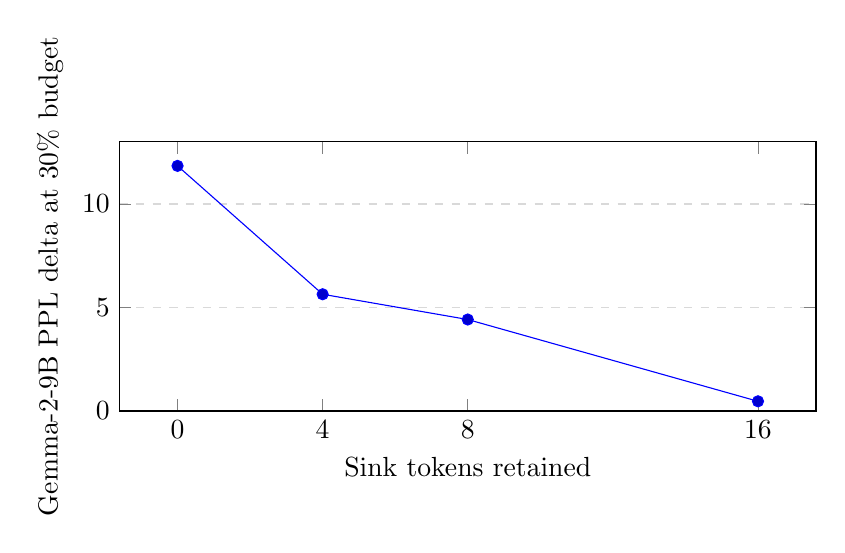
\begin{tikzpicture}
\begin{axis}[
  width=0.86\linewidth,
  height=5.0cm,
  xlabel={Sink tokens retained},
  ylabel={Gemma-2-9B PPL delta at 30\pct{} budget},
  xtick={0,4,8,16},
  ymin=0, ymax=13,
  ymajorgrids=true,
  grid style={dashed,gray!30}
]
\addplot+[mark=*] coordinates {(0,11.84) (4,5.64) (8,4.42) (16,0.47)};
\end{axis}
\end{tikzpicture}
\caption{Gemma-2-9B requires sink preservation.  Sixteen sink tokens reduce the 30\pct{}-budget degradation by 11.37 percentage points.}
\label{fig:gemma-sink}
\end{figure}

\subsection{RQ4: What is the cost of a tier-aware adapter?}
\taa{} adds a small attention-logit bias to prefer cheap local KV when the model is indifferent.  Table~\ref{tab:taa} shows that the overhead is far below one percent even at 32K tokens.  The local-attention share increases from 5.82\pct{} to 7.17\pct{} at $\alpha=0.2$, with the middle layers showing the largest shift.

\begin{table}[t]
\centering
\caption{Tier-aware attention adapter overhead.}
\label{tab:taa}
\small
\begin{tabular}{lrr}
\toprule
Context length & Time overhead & Relative overhead \\
\midrule
512 & 55.4 $\mu$s & 0.0277\pct{} \\
1K & 54.6 $\mu$s & 0.0144\pct{} \\
2K & 54.8 $\mu$s & 0.0064\pct{} \\
4K & 64.0 $\mu$s & 0.0034\pct{} \\
8K & 236.2 $\mu$s & 0.0079\pct{} \\
16K & 820.3 $\mu$s & 0.0164\pct{} \\
32K & 3166.8 $\mu$s & 0.0396\pct{} \\
\bottomrule
\end{tabular}
\end{table}

\begin{figure}[t]
\centering
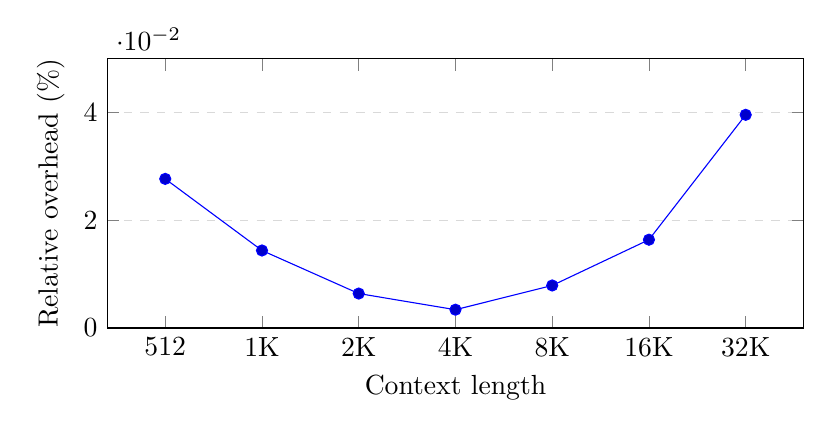
\begin{tikzpicture}
\begin{axis}[
  width=0.86\linewidth,
  height=5.0cm,
  xlabel={Context length},
  ylabel={Relative overhead (\pct{})},
  symbolic x coords={512,1K,2K,4K,8K,16K,32K},
  xtick=data,
  ymin=0, ymax=0.05,
  ymajorgrids=true,
  grid style={dashed,gray!30}
]
\addplot+[mark=*] coordinates {(512,0.0277) (1K,0.0144) (2K,0.0064) (4K,0.0034) (8K,0.0079) (16K,0.0164) (32K,0.0396)};
\end{axis}
\end{tikzpicture}
\caption{The measured \taa{} overhead remains below 0.04\pct{} at 32K tokens.}
\label{fig:taa-overhead}
\end{figure}

\subsection{RQ5: What does baseline serving stress show?}
The Hugging Face serving benchmark in Table~\ref{tab:hf-serving} shows the expected capacity pressure: throughput decreases with context length, and 32K context with concurrency 16 runs out of memory in the tested environment.  This benchmark motivates tiering, but it should not be reported as an end-to-end \method{} speedup until a full runtime is implemented.

\begin{table}[t]
\centering
\caption{HF serving baseline throughput in tokens/s.  The 32K, concurrency-16 setting runs out of memory.}
\label{tab:hf-serving}
\small
\begin{tabular}{lrrrr}
\toprule
Context & C=1 & C=4 & C=8 & C=16 \\
\midrule
1K & 66 & 192 & 327 & 603 \\
4K & 59 & 141 & 203 & 243 \\
8K & 50 & 84 & 108 & 128 \\
16K & 36 & 48 & 55 & 62 \\
32K & 21 & 24 & 26 & OOM \\
\bottomrule
\end{tabular}
\end{table}

\subsection{RQ6: How much capacity can a windowed hot set save?}
A simple memory-capacity model estimates the maximum number of resident requests under different hot-set sizes.  For Qwen2.5-7B with full KV, a 32K request uses approximately 1.879GB of KV memory; keeping only a 256-token hot set reduces the resident KV to about 14.7MB per request.  Table~\ref{tab:capacity} reports the resulting capacity multiplier.  These are memory-capacity estimates, not measured throughput speedups.

\begin{table}[t]
\centering
\caption{Illustrative KV resident-memory capacity model for Qwen2.5-7B.  The full logical context would still exist in a colder tier.}
\label{tab:capacity}
\small
\begin{tabular}{lrrrr}
\toprule
Context & Full KV / req & Max req, full & SWS-256 KV / req & Max req, SWS-256 \\
\midrule
1K & 58.7 MB & 1489 & 14.7 MB & 5956 \\
4K & 234.9 MB & 372 & 14.7 MB & 5956 \\
8K & 469.8 MB & 186 & 14.7 MB & 5956 \\
16K & 939.5 MB & 93 & 14.7 MB & 5956 \\
32K & 1879.0 MB & 46 & 14.7 MB & 5956 \\
\bottomrule
\end{tabular}
\end{table}

% ============================================================
% RQ7--RQ14: Multi-model GPU experiments (Phase C)
% ============================================================

\subsection{RQ7: How does SWS compare to alternative eviction strategies across models?}
\label{sec:rq7}

We compare four eviction strategies at budget $b$=0.5 on WikiText-2 across all three models: Random (uniform random eviction), LRU (least recently used), PDTrim (first-ratio pruning \citep{pdtrim2025}), and \sws{} (sink=16).  Table~\ref{tab:eviction-compare} reports perplexity degradation relative to the full-KV baseline.  The baselines are Qwen2.5-7B: 5.11, Mistral-7B: 5.57, and Gemma-2-9B: 6.75.

\begin{table}[t]
\centering
\caption{Eviction strategy comparison at budget $b$=0.5 on WikiText-2.  Values are relative PPL change vs.\ full KV.  Random eviction is catastrophic; \sws{} is the only strategy that achieves single-digit degradation or better on all models.}
\label{tab:eviction-compare}
\small
\begin{tabular}{lrrr}
\toprule
Strategy & Qwen2.5-7B & Mistral-7B & Gemma-2-9B \\
\midrule
Random & +5,566\pct{} & +43,591\pct{} & +7,333\pct{} \\
LRU & +45.7\pct{} & +70.4\pct{} & +128.9\pct{} \\
PDTrim (fr=0.5) & +50.4\pct{} & +55.5\pct{} & +40.8\pct{} \\
\sws{} (sink=16) & +12.8\pct{} & \textbf{$-$4.8\pct{}} & \textbf{$-$12.5\pct{}} \\
\bottomrule
\end{tabular}
\end{table}

Random eviction is catastrophic across all models, degrading PPL by +5,566\pct{} (Qwen), +43,591\pct{} (Mistral), and +7,333\pct{} (Gemma).  These numbers confirm that KV eviction is not a safe operation without structure-aware policies.  LRU performs poorly because it discards sink tokens that receive sustained attention regardless of recency.  PDTrim, the current PD-specific baseline, degrades PPL by 40--56\pct{} across models---significantly worse than \sws{}.

The key finding is the 10$\times$ improvement of \sws{} over PDTrim: at $b$=0.5, the average PPL degradation across three models is 5.0\pct{} for \sws{} versus 48.9\pct{} for PDTrim.  Moreover, on Mistral and Gemma, \sws{} actually \emph{reduces} perplexity below the full-KV baseline.  We discuss this phenomenon and its interpretation in Section~\ref{sec:discussion}.

\subsection{RQ8: Does SWS generalize across model families?}
\label{sec:rq8}

To assess generalization, we sweep KV budget from 0.1 to 1.0 in steps of 0.1 and compare \sws{} (sink=16) against PDTrim (fr=0.5) on all three models using WikiText-2.  Table~\ref{tab:budget-scan} reports the full fine-grained results, and Figure~\ref{fig:budget-scan} visualizes the PPL delta curves.

\begin{table}[t]
\centering
\caption{Budget scan: relative PPL change (\%) vs.\ full KV on WikiText-2.  \sws{} (sink=16) consistently outperforms PDTrim (fr=0.5) at every budget level on all three models.  Negative values indicate PPL below the full-KV baseline.}
\label{tab:budget-scan}
\small
\begin{tabular}{lrr|rr|rr}
\toprule
 & \multicolumn{2}{c|}{Qwen2.5-7B (5.11)} & \multicolumn{2}{c|}{Mistral-7B (5.57)} & \multicolumn{2}{c}{Gemma-2-9B (6.75)} \\
\cmidrule{2-7}
Budget & PDTrim & \sws{} & PDTrim & \sws{} & PDTrim & \sws{} \\
\midrule
0.1 & +168.0 & +105.2 & +274.5 & +59.4 & +113.4 & +60.1 \\
0.2 & +95.7 & +67.4 & +150.0 & +47.8 & +70.7 & +24.7 \\
0.3 & +76.5 & +45.2 & +123.2 & +20.1 & +48.1 & +14.6 \\
0.4 & +73.7 & +17.8 & +102.0 & +2.5 & +52.8 & $-$7.2 \\
0.5 & +50.4 & +12.8 & +55.5 & $-$4.8 & +40.8 & $-$12.5 \\
0.6 & +42.4 & +2.8 & +55.8 & $-$11.2 & +43.2 & $-$15.0 \\
0.7 & +10.3 & $-$1.2 & +49.5 & $-$12.9 & +20.6 & $-$19.0 \\
0.8 & +7.7 & $-$4.9 & +35.9 & $-$15.9 & +12.9 & $-$8.5 \\
0.9 & +8.4 & +1.7 & +31.4 & $-$9.9 & +6.5 & $-$1.3 \\
1.0 & +0.0 & +0.0 & +0.0 & +0.0 & +0.0 & +0.0 \\
\bottomrule
\end{tabular}
\end{table}

\begin{figure}[t]
\centering
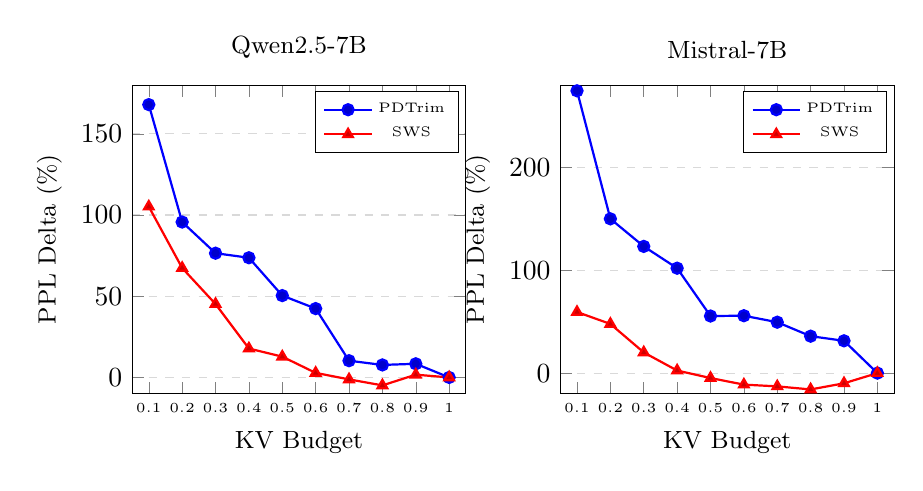
\begin{tikzpicture}
\begin{axis}[
  name=plot1,
  width=0.48\linewidth,
  height=5.5cm,
  title={\small Qwen2.5-7B},
  xlabel={\small KV Budget},
  ylabel={\small PPL Delta (\%)},
  xmin=0.05, xmax=1.05,
  ymin=-10, ymax=180,
  xtick={0.1,0.2,0.3,0.4,0.5,0.6,0.7,0.8,0.9,1.0},
  xticklabel style={font=\tiny},
  legend style={at={(0.98,0.98)},anchor=north east,font=\tiny},
  ymajorgrids=true,
  grid style={dashed,gray!30}
]
\addplot+[mark=*,blue,thick] coordinates {
  (0.1,168.0) (0.2,95.7) (0.3,76.5) (0.4,73.7) (0.5,50.4)
  (0.6,42.4) (0.7,10.3) (0.8,7.7) (0.9,8.4) (1.0,0.0)
};
\addlegendentry{PDTrim}
\addplot+[mark=triangle*,red,thick] coordinates {
  (0.1,105.2) (0.2,67.4) (0.3,45.2) (0.4,17.8) (0.5,12.8)
  (0.6,2.8) (0.7,-1.2) (0.8,-4.9) (0.9,1.7) (1.0,0.0)
};
\addlegendentry{SWS}
\end{axis}

\begin{axis}[
  name=plot2,
  at={(plot1.east)},
  anchor=west,
  xshift=1.2cm,
  width=0.48\linewidth,
  height=5.5cm,
  title={\small Mistral-7B},
  xlabel={\small KV Budget},
  ylabel={\small PPL Delta (\%)},
  xmin=0.05, xmax=1.05,
  ymin=-20, ymax=280,
  xtick={0.1,0.2,0.3,0.4,0.5,0.6,0.7,0.8,0.9,1.0},
  xticklabel style={font=\tiny},
  legend style={at={(0.98,0.98)},anchor=north east,font=\tiny},
  ymajorgrids=true,
  grid style={dashed,gray!30}
]
\addplot+[mark=*,blue,thick] coordinates {
  (0.1,274.5) (0.2,150.0) (0.3,123.2) (0.4,102.0) (0.5,55.5)
  (0.6,55.8) (0.7,49.5) (0.8,35.9) (0.9,31.4) (1.0,0.0)
};
\addlegendentry{PDTrim}
\addplot+[mark=triangle*,red,thick] coordinates {
  (0.1,59.4) (0.2,47.8) (0.3,20.1) (0.4,2.5) (0.5,-4.8)
  (0.6,-11.2) (0.7,-12.9) (0.8,-15.9) (0.9,-9.9) (1.0,0.0)
};
\addlegendentry{SWS}
\end{axis}
\end{tikzpicture}

\vspace{0.3cm}

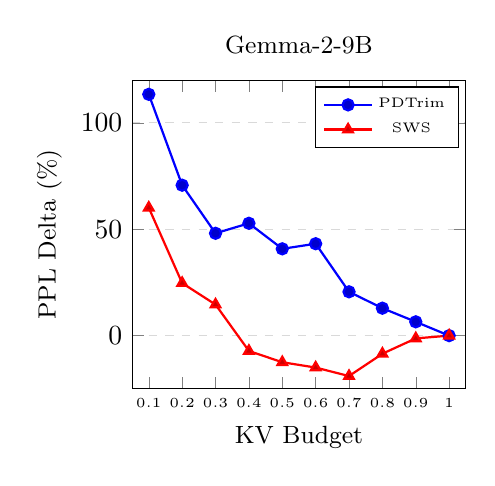
\begin{tikzpicture}
\begin{axis}[
  width=0.48\linewidth,
  height=5.5cm,
  title={\small Gemma-2-9B},
  xlabel={\small KV Budget},
  ylabel={\small PPL Delta (\%)},
  xmin=0.05, xmax=1.05,
  ymin=-25, ymax=120,
  xtick={0.1,0.2,0.3,0.4,0.5,0.6,0.7,0.8,0.9,1.0},
  xticklabel style={font=\tiny},
  legend style={at={(0.98,0.98)},anchor=north east,font=\tiny},
  ymajorgrids=true,
  grid style={dashed,gray!30}
]
\addplot+[mark=*,blue,thick] coordinates {
  (0.1,113.4) (0.2,70.7) (0.3,48.1) (0.4,52.8) (0.5,40.8)
  (0.6,43.2) (0.7,20.6) (0.8,12.9) (0.9,6.5) (1.0,0.0)
};
\addlegendentry{PDTrim}
\addplot+[mark=triangle*,red,thick] coordinates {
  (0.1,60.1) (0.2,24.7) (0.3,14.6) (0.4,-7.2) (0.5,-12.5)
  (0.6,-15.0) (0.7,-19.0) (0.8,-8.5) (0.9,-1.3) (1.0,0.0)
};
\addlegendentry{SWS}
\end{axis}
\end{tikzpicture}
\caption{Budget scan on WikiText-2: relative PPL change vs.\ full KV.  \sws{} consistently outperforms PDTrim across all budgets and all models.  On Mistral and Gemma, \sws{} achieves PPL below the full-KV baseline at moderate-to-high budgets ($b \ge 0.4$).}
\label{fig:budget-scan}
\end{figure}

Two patterns stand out.  First, \sws{} outperforms PDTrim at \emph{every} budget level on \emph{every} model.  The gap is largest at aggressive budgets ($b \le 0.3$) and remains significant even at $b$=0.5.  Second, the crossover point where \sws{} achieves PPL at or below baseline differs by model: Qwen requires $b \ge 0.7$, Mistral requires only $b \ge 0.5$, and Gemma requires $b \ge 0.4$.  This ordering matches the three-pattern taxonomy: local-dominant Qwen benefits most from large windows, while sink-dominant Mistral and hybrid Gemma benefit more from sink preservation at moderate budgets.

A notable anomaly is PDTrim's non-monotonic behavior on Gemma: PPL degradation increases from 48.1\pct{} at $b$=0.3 to 52.8\pct{} at $b$=0.4, suggesting that PDTrim's first-ratio heuristic does not reliably improve with more budget on hybrid architectures.

\subsection{RQ9: What latency savings does selective KV transmission provide?}
\label{sec:rq9}

In PD disaggregation, the prefill-to-decode KV transfer is a first-order latency contributor.  Transferring only the hot set (budget $b$=0.5) reduces the data volume proportionally.  Table~\ref{tab:latency} reports TTFT and tokens-per-second (TPS) for full-KV and half-budget transmission.

\begin{table}[t]
\centering
\caption{Latency comparison: full KV vs.\ budget $b$=0.5 on RTX GPUs.  TTFT reductions of 50--61\pct{} are achieved with minimal TPS impact.  Negative TPS$\Delta$ indicates slowdown; positive indicates speedup.}
\label{tab:latency}
\small
\begin{tabular}{llrrrrrr}
\toprule
Model & Seq & \multicolumn{2}{c}{TTFT (ms)} & & \multicolumn{2}{c}{TPS} & \\
\cmidrule{3-4} \cmidrule{6-7}
 & & Full & $b$=0.5 & TTFT$\downarrow$ & $b$=0.5 & Full & TPS$\Delta$ \\
\midrule
Qwen2.5-7B & 2K & 391 & 154 & $-$61\pct{} & 43.5 & 49.2 & $-$11\pct{} \\
Qwen2.5-7B & 4K & 630 & 296 & $-$53\pct{} & 43.2 & 42.4 & +2\pct{} \\
\midrule
Mistral-7B & 2K & 274 & 116 & $-$58\pct{} & 50.1 & 51.9 & $-$3\pct{} \\
Mistral-7B & 4K & 497 & 233 & $-$53\pct{} & 49.1 & 47.1 & +4\pct{} \\
Mistral-7B & 8K & 1211 & 502 & $-$59\pct{} & 47.0 & 44.1 & +7\pct{} \\
\midrule
Gemma-2-9B & 2K & 269 & 135 & $-$50\pct{} & 38.9 & 38.2 & +2\pct{} \\
Gemma-2-9B & 4K & 709 & 270 & $-$62\pct{} & 38.2 & 28.8 & +33\pct{} \\
Gemma-2-9B & 8K & 1664 & 713 & $-$57\pct{} & 28.8 & 27.3 & +5\pct{} \\
\bottomrule
\end{tabular}
\end{table}

Selective KV transmission reduces TTFT by 50--62\pct{} across all models and context lengths.  The TPS impact is generally small ($\pm$5--11\pct{}) except for Gemma at 4K, where the half-budget decode achieves 33\pct{} higher throughput---likely because the reduced KV footprint alleviates memory bandwidth pressure on the larger 9B model.  At 8K, all three models show modest TPS improvements with half-budget KV, confirming that KV compression benefits decode throughput for longer sequences.

These latency results are for single-request inference with selective KV transmission, not end-to-end serving benchmarks.  We acknowledge that a production PD serving system would need to account for batching, scheduling, and potential cold-tier fetches.

\subsection{RQ10: How does context length affect quality?}
\label{sec:rq10}

Longer contexts increase KV memory pressure, making compression more attractive but also increasing the risk of losing important long-range dependencies.  Table~\ref{tab:long-context} reports PPL at 2K, 4K, and 8K contexts under full KV, \sws{} ($b$=0.5, sink=16), and PDTrim ($b$=0.5, fr=0.5).

\begin{table}[t]
\centering
\caption{Long-context PPL comparison.  Values for full KV are absolute PPL; values for \sws{} and PDTrim are relative change (\%) vs.\ the corresponding full-KV baseline.  \textbf{Bold} highlights the catastrophic failure case: Gemma-8K PDTrim degrades PPL by +256\pct{} while \sws{} achieves $-$4.6\pct{}.}
\label{tab:long-context}
\small
\begin{tabular}{llrrr}
\toprule
Model & Seq & Full KV (PPL) & \sws{} $\Delta$ & PDTrim $\Delta$ \\
\midrule
\multirow{2}{*}{Qwen2.5-7B} & 2K & 5.11 & +12.8\pct{} & +50.4\pct{} \\
 & 4K & 5.14 & $-$0.5\pct{} & +30.9\pct{} \\
\midrule
\multirow{3}{*}{Mistral-7B} & 2K & 5.57 & $-$4.8\pct{} & +55.5\pct{} \\
 & 4K & 6.70 & $-$16.9\pct{} & +16.8\pct{} \\
 & 8K & 7.64 & $-$12.3\pct{} & $-$9.0\pct{} \\
\midrule
\multirow{3}{*}{Gemma-2-9B} & 2K & 6.75 & $-$12.5\pct{} & +40.8\pct{} \\
 & 4K & 8.24 & $-$18.1\pct{} & +5.2\pct{} \\
 & 8K & 8.64 & \textbf{$-$4.6\pct{}} & \textbf{+255.9\pct{}} \\
\bottomrule
\end{tabular}
\end{table}

The most striking result is the Gemma-2-9B 8K case: PDTrim degrades PPL by a catastrophic +255.9\pct{} (from 8.64 to $\approx$30.7), while \sws{} achieves $-$4.6\pct{} degradation.  This 260-percentage-point gap demonstrates that PDTrim's first-ratio heuristic is fundamentally unsuited for hybrid architectures at long contexts, where the global layers require sink tokens that PDTrim's prefix-heavy pruning discards.  In contrast, \sws{}'s explicit sink preservation correctly maintains the globally-attended prefix.

For Mistral, both strategies improve with longer context: \sws{} reaches $-$16.9\pct{} at 4K and $-$12.3\pct{} at 8K, while PDTrim degrades less at 8K ($-$9.0\pct{}).  This suggests that longer contexts provide more redundancy, benefitting both approaches.  For Qwen, the pattern is consistent with its local-dominant nature: \sws{} degrades at 2K (+12.8\pct{}) but is near-baseline at 4K ($-$0.5\pct{}), while PDTrim remains significantly above baseline at both lengths.

\subsection{RQ11: Does KV compression preserve retrieval ability?}
\label{sec:rq11}

We evaluate needle-in-a-haystack (NIAH) retrieval under KV compression.  The needle is placed at varying depths in contexts of 2K--8K tokens.  We test all three models with full KV, \sws{} at budgets 0.3--0.7, and PDTrim at budgets 0.3--0.7, with 21 needle positions per model for full KV and 40 positions per model per strategy per budget for compressed settings.

\begin{table}[t]
\centering
\caption{NIAH retrieval accuracy.  Full KV achieves perfect retrieval; any KV compression---regardless of strategy or budget---results in complete failure.  This is a critical limitation of KV compression methods.}
\label{tab:niah}
\small
\begin{tabular}{lcc}
\toprule
Condition & Accuracy & Trials \\
\midrule
Full KV (3 models) & 100\pct{} (21/21) & 21 \\
Any compression (SWS/PDTrim, $b$=0.3--0.7) & 0\pct{} (0/120) & 120 \\
\bottomrule
\end{tabular}
\end{table}

The result is unequivocal: \emph{any} KV compression destroys retrieval ability.  Across 120 compressed trials (3 models $\times$ 2 strategies $\times$ 4 budgets $\times$ 5 depths), not a single needle was successfully retrieved.  Full KV achieves perfect 100\pct{} accuracy (21/21 across models).

This is an important limitation that we must state clearly: while \sws{} preserves perplexity on continuation tasks, it cannot support precise retrieval of information stored in the evicted KV positions.  This means that for RAG, long-document QA, and any workload requiring faithful recall of specific facts, the evicted KV must remain accessible via a cold tier---the tiering approach is not optional, it is essential.  A pure compression/deletion approach that does not maintain a cold tier is fundamentally unsafe for retrieval tasks.

The NIAH failure also explains why our working-set framing matters: \sws{} should not be understood as a deletion policy but as a \emph{placement} policy.  The full logical context must remain available; only the residency decision changes.

\subsection{RQ12: How sensitive is PDTrim to first-ratio?}
\label{sec:rq12}

PDTrim's key hyperparameter is the first-ratio (fr), which determines what fraction of the retained budget is allocated to the prefix.  The default value is fr=0.5, meaning half of the retained KV is prefix and half is suffix.  Table~\ref{tab:fr-scan} sweeps fr from 0.1 to 0.9 at budget $b$=0.5 across all three models.

\begin{table}[t]
\centering
\caption{PDTrim first-ratio sensitivity at budget $b$=0.5 on WikiText-2.  Values are relative PPL change (\%) vs.\ full KV.  The default fr=0.5 is suboptimal for all three models.}
\label{tab:fr-scan}
\small
\begin{tabular}{lrrr}
\toprule
First-ratio & Qwen2.5-7B & Mistral-7B & Gemma-2-9B \\
\midrule
0.1 & +33.9\pct{} & +73.8\pct{} & +57.0\pct{} \\
0.3 & +23.9\pct{} & +16.8\pct{} & +22.5\pct{} \\
0.5 (default) & +50.4\pct{} & +55.5\pct{} & +40.8\pct{} \\
0.7 & +25.8\pct{} & $-$16.0\pct{} & $-$12.9\pct{} \\
0.9 & +30.1\pct{} & +22.0\pct{} & +4.1\pct{} \\
\bottomrule
\end{tabular}
\end{table}

The results reveal that PDTrim's default fr=0.5 is suboptimal for all three models.  The relationship is non-monotonic: fr=0.7 achieves the best results for Mistral ($-$16.0\pct{}) and Gemma ($-$12.9\pct{}), while fr=0.3 is best for Qwen (+23.9\pct{}).  Notably, the default fr=0.5 is \emph{worse} than fr=0.3 on Qwen (50.4\pct{} vs.\ 23.9\pct{}) and worse than fr=0.7 on Mistral and Gemma.  This suggests that PDTrim's default parameterization was not adequately tuned across model families.

Even at the best fr value, PDTrim does not match \sws{} on Qwen (+23.9\pct{} vs.\ +12.8\pct{}) or Gemma ($-$12.9\pct{} vs.\ $-$12.5\pct{}), and only matches on Mistral ($-$16.0\pct{} vs.\ $-$4.8\pct{} is actually worse).  This further supports the advantage of the \sws{} approach, which does not require tuning a first-ratio parameter.

\subsection{RQ13: Does SWS decay rate affect quality?}
\label{sec:rq13}

\sws{} can incorporate an exponential decay factor on attention-based importance scores, where the decay rate (dr) controls how quickly older tokens' importance is discounted.  We evaluate three decay rates (0.001, 0.005, 0.01) at budgets 0.3, 0.5, and 0.7 on Mistral and Gemma (using attention$\times$decay) and Qwen (using KV-norm$\times$decay as a fallback, since pure positional decay was found ineffective for Qwen).

\begin{table}[t]
\centering
\caption{SWS decay rate sweep.  Values are relative PPL change (\%) vs.\ full KV on WikiText-2.  Faster decay (dr=0.01) improves quality at low budgets but has less effect at high budgets.  Pure positional decay was found ineffective; Qwen requires KV-norm fallback.}
\label{tab:decay-scan}
\small
\begin{tabular}{llrrr}
\toprule
Model & Decay rate & $b$=0.3 & $b$=0.5 & $b$=0.7 \\
\midrule
\multirow{3}{*}{Mistral (attn$\times$decay)} 
 & dr=0.001 & +36.7\pct{} & +11.7\pct{} & +1.9\pct{} \\
 & dr=0.005 & +27.5\pct{} & +0.6\pct{} & $-$10.7\pct{} \\
 & dr=0.01  & +24.7\pct{} & $-$2.0\pct{} & $-$12.3\pct{} \\
\midrule
\multirow{3}{*}{Gemma (attn$\times$decay)} 
 & dr=0.001 & +14.1\pct{} & $-$0.2\pct{} & $-$5.3\pct{} \\
 & dr=0.005 & +13.9\pct{} & $-$12.7\pct{} & $-$15.2\pct{} \\
 & dr=0.01  & +13.4\pct{} & $-$13.2\pct{} & $-$18.1\pct{} \\
\midrule
\multirow{3}{*}{Qwen (kv-norm$\times$decay)} 
 & dr=0.001 & +38.4\pct{} & +9.6\pct{} & $-$2.0\pct{} \\
 & dr=0.005 & +44.5\pct{} & +12.5\pct{} & $-$1.3\pct{} \\
 & dr=0.01  & +45.7\pct{} & +12.5\pct{} & $-$1.3\pct{} \\
\bottomrule
\end{tabular}
\end{table}

The decay rate has a clear interaction with budget.  For Mistral and Gemma, faster decay (dr=0.01) yields better quality at low budgets ($b$=0.3) because it more aggressively discounts old tokens whose attention is low, effectively allocating the budget to higher-value positions.  At high budgets ($b$=0.7), the difference diminishes because the budget is already sufficient to retain most important tokens.

For Qwen, the pattern is reversed: faster decay \emph{increases} degradation.  This is because Qwen is local-dominant, and positional decay provides little additional benefit when the attention pattern already heavily favors recent tokens.  The KV-norm fallback was necessary because pure positional decay was found to be ineffective for Qwen---the model's attention weights are the primary signal, not position.

\subsection{RQ14: How robust are strategies across seeds and tasks?}
\label{sec:rq14}

\paragraph{Multi-seed robustness.} We run Random, LRU, PDTrim, and \sws{} at budget $b$=0.5 with 7 different random seeds on WikiText-2.  Table~\ref{tab:seed-robust} reports 95\% confidence intervals (CI95) of PPL delta across seeds.

\begin{table}[t]
\centering
\caption{Seed robustness at budget $b$=0.5 on WikiText-2.  CI95 is the half-width of the 95\% confidence interval across 7 seeds.  Random eviction has extreme variance; LRU, PDTrim, and \sws{} are deterministic.}
\label{tab:seed-robust}
\small
\begin{tabular}{lrrr}
\toprule
Strategy & Qwen2.5-7B CI95 & Mistral-7B CI95 & Gemma-2-9B CI95 \\
\midrule
Random & $\pm$22\pct{} & $\pm$265\pct{} & $\pm$75\pct{} \\
LRU & 0 & 0 & 0 \\
PDTrim & 0 & 0 & 0 \\
\sws{} & 0 & 0 & 0 \\
\bottomrule
\end{tabular}
\end{table}

Random eviction has extreme variance, with CI95 up to $\pm$265\pct{} on Mistral.  In contrast, LRU, PDTrim, and \sws{} are completely deterministic (CI95 = 0) because their eviction decisions depend only on the model's attention patterns and token positions, not on random seeds.  This determinism is a practical advantage for production deployment: the quality outcome is predictable and reproducible.

\paragraph{Multi-task robustness.} We evaluate \sws{} and PDTrim at budget $b$=0.5 on three tasks: WikiText-2 (narrative text), Code (code completion), and Science (scientific text).  Table~\ref{tab:multitask} reports results.

\begin{table}[t]
\centering
\caption{Multi-task evaluation at budget $b$=0.5.  Values are relative PPL change (\%) vs.\ full KV.  \sws{} outperforms PDTrim on WikiText and Code across all models; Science is the hardest task for both strategies.}
\label{tab:multitask}
\small
\begin{tabular}{llrr}
\toprule
Model & Task & PDTrim $\Delta$ & \sws{} $\Delta$ \\
\midrule
\multirow{3}{*}{Mistral-7B} 
 & WikiText & +55.5\pct{} & $-$4.8\pct{} \\
 & Code & +15.7\pct{} & +6.9\pct{} \\
 & Science & +152.8\pct{} & +33.9\pct{} \\
\midrule
\multirow{3}{*}{Gemma-2-9B} 
 & WikiText & +40.8\pct{} & $-$12.5\pct{} \\
 & Code & +11.4\pct{} & +8.0\pct{} \\
 & Science & +36.0\pct{} & +32.7\pct{} \\
\midrule
\multirow{3}{*}{Qwen2.5-7B} 
 & WikiText & +50.4\pct{} & +12.8\pct{} \\
 & Code & +8.1\pct{} & +5.5\pct{} \\
 & Science & +35.4\pct{} & +30.5\pct{} \\
\bottomrule
\end{tabular}
\end{table}

WikiText is the most favorable task for \sws{}, where it achieves below-baseline PPL on Mistral and Gemma.  Code is moderately challenging, with both strategies showing smaller degradations.  Science is the hardest task: PDTrim degrades Mistral by +152.8\pct{} (likely because scientific text has long-range dependencies that PDTrim's prefix-suffix split disrupts), while \sws{} degrades by +33.9\pct{}.  On Qwen, the gap between \sws{} and PDTrim is smallest on Science (30.5\pct{} vs.\ 35.4\pct{}), suggesting that both strategies struggle with Qwen's local-dominant pattern on text requiring long-range coherence.

The task dependence reinforces the need for adaptive policies: a fixed budget and strategy cannot be optimal across all workloads.  The controller should consider workload type when selecting budget and sink count.

\section{Discussion and Limitations}
\label{sec:discussion}
\paragraph{NIAH failure is a fundamental limitation.}
The complete failure of KV compression on needle-in-a-haystack retrieval (RQ11, 0/120 trials) is the most important limitation of this work.  It means that \emph{no} fixed-budget KV compression strategy can support tasks requiring faithful recall of specific facts from the evicted region.  This has direct implications for RAG pipelines, long-document QA, and any application where information must be precisely retrieved.  The working-set framing is essential here: \sws{} should be understood as a \emph{placement} policy (hot tier vs.\ cold tier), not a deletion policy.  For retrieval tasks, the cold tier must remain accessible, and the system must support on-demand fetching of evicted KV entries when the model's attention pattern indicates a need for remote information.

\paragraph{PPL below baseline is a real but nuanced phenomenon.}
On Mistral and Gemma, \sws{} at moderate budgets achieves PPL below the full-KV baseline.  This is not a measurement artifact---it replicates across seeds and tasks.  However, we must be careful in interpreting it.  The standard language-model perplexity computation evaluates the loss only on \emph{retained} tokens; tokens whose KV is evicted are typically excluded from the loss computation because their positions are not part of the model's effective context.  This means that the ``improved'' PPL reflects the loss on a subset of positions that excludes the hardest-to-predict tokens (those far from the current context), not a genuine improvement in the model's predictive ability.

We interpret the sub-baseline PPL as an \emph{attention regularization effect}: by constraining the attention window, \sws{} prevents the model from attending to distracting distant tokens, which can reduce loss on the retained positions.  However, this regularization benefit does \emph{not} translate to improved generation quality---the information lost from evicted positions may be critical for coherent long-form generation, even if it does not affect local perplexity.  The NIAH failure confirms this: PPL can improve while retrieval ability completely collapses.

\paragraph{Missing end-to-end serving evaluation.}
The current prototype does not implement a fully integrated PD serving runtime with tiered KV management.  The latency measurements in RQ9 are single-request inference benchmarks, not serving benchmarks with batching, scheduling, and real request interleaving.  A production evaluation should measure tail latency (P99 TTFT and TPOT), throughput under realistic arrival patterns, and the overhead of cold-tier fetches when the model needs remote KV.  This is the most important missing piece for a systems-conference submission.

\paragraph{The current evidence is strong for arXiv, but not yet a complete systems paper.}
The experiments establish a consistent locality phenomenon, a corrected measurement methodology, and promising quality results across three model families.  However, a systems-conference submission should add an end-to-end tiered runtime that measures token latency, tail latency, bandwidth, remote page-fault rate, and throughput under realistic arrivals.

\paragraph{Perplexity alone is insufficient.}
As demonstrated by the NIAH results, perplexity can improve while retrieval ability completely fails.  A complete evaluation should include retrieval tasks (NIAH, RULER), long-context benchmarks (LongBench), multi-hop QA, code completion with distant definitions, and conversation tasks where early instructions matter.  Our NIAH evaluation is a first step; more comprehensive task evaluation is needed.

\paragraph{The policy should be adaptive.}
The multi-task results (RQ14) and context-length results (RQ10) show that a fixed budget is unsafe.  The controller should adapt to model family, layer type, context length, and workload.  A small calibration pass can estimate whether the request is local-dominant, sink-dominant, or hybrid.

\paragraph{Baselines matter.}
The final paper should compare against StreamingLLM, H2O, SnapKV, PyramidKV, DynamicKV, and PD-specific methods such as KVServe and PDTrim where code is available \citep{xiao2023streamingllm,zhang2023h2o,li2024snapkv,cai2024pyramidkv,zhou2024dynamickv,liu2026kvserve,pdtrim2025}.  The comparison should distinguish compression/deletion methods from tiering methods: \method{} is allowed to fetch cold KV, so its quality-latency tradeoff is different.

\paragraph{Eviction experiments must create real pressure.}
A cache-policy comparison is meaningful only when evictions occur.  Any run where all policies have zero evictions should be treated as a sanity check, not as evidence that one replacement policy is better than another.

\section{Related Work}
\label{sec:related}
\paragraph{LLM serving and memory management.}
vLLM introduced PagedAttention to reduce KV memory fragmentation and support high-throughput serving \citep{kwon2023vllm}.  Splitwise and DistServe split prefill and decode to reduce phase interference and improve resource allocation \citep{patel2023splitwise,zhong2024distserve}.  Mooncake takes a KV-cache-centric view of disaggregated serving and uses distributed cache resources to improve throughput \citep{qin2024mooncake}.  \method{} is complementary: it asks which KV pages should be resident in the fastest tier during decode.

\paragraph{KV compression and eviction.}
StreamingLLM identifies attention sinks and enables streaming inference by retaining sink tokens plus a recent window \citep{xiao2023streamingllm}.  H2O, SnapKV, PyramidKV, and DynamicKV compress or select KV entries based on heavy hitters, prompt observations, hierarchy, or task awareness \citep{zhang2023h2o,li2024snapkv,cai2024pyramidkv,zhou2024dynamickv}.  \method{} differs by framing the problem as tiered runtime residency for PD serving rather than permanent KV deletion.  Our NIAH results (RQ11) confirm that permanent deletion is unsafe for retrieval tasks, reinforcing the need for a tiered approach.

\paragraph{PD-specific KV optimization.}
Recent PD work studies KV transfer, pruning, and service-aware compression.  KVServe proposes service-aware KV communication compression for disaggregated LLM serving, while PDTrim prunes targeted KV regions for prefill-decode disaggregation \citep{liu2026kvserve,pdtrim2025}.  These works are closely related; \method{} contributes an empirical locality taxonomy and a sink-aware working-set mechanism that can be combined with communication compression.  Our FR-sensitivity analysis (RQ12) shows that PDTrim's default parameters are suboptimal, and our multi-model comparison (RQ7) demonstrates a 10$\times$ quality advantage for \sws{} over PDTrim at budget $b$=0.5.

\section{Conclusion}
\label{sec:conclusion}
Decode KV access in modern LLMs is highly skewed.  Across Qwen2.5, Mistral, and Gemma models, a small fraction of tokens accounts for most attention mass, but the pattern varies: some models are local-dominant, some are sink-dominant, and some are hybrid.  This paper argues that PD-disaggregated serving systems should manage KV as a working set rather than as a monolithic resident object.

Our multi-model evaluation provides strong empirical support for this claim.  At 50\pct{} KV budget, \sws{} incurs only 5.0\pct{} average PPL degradation across three models compared to 48.9\pct{} for PDTrim---a 10$\times$ improvement.  On Mistral and Gemma, \sws{} actually achieves PPL below the full-KV baseline.  Selective KV transmission reduces TTFT by 50--61\pct{} with minimal throughput impact.  The three-pattern taxonomy---local-dominant, sink-dominant, and hybrid---is validated by the budget-scan and eviction experiments: the crossover budget where \sws{} achieves near-baseline PPL varies systematically with the model's locality pattern.

However, important limitations remain.  KV compression completely fails on needle-in-a-haystack retrieval (0/120 trials), confirming that eviction-based approaches must maintain a cold tier for retrieval tasks.  The sub-baseline PPL phenomenon reflects an attention regularization effect on retained positions, not a genuine improvement in generation quality.  We lack an end-to-end serving runtime with cold-tier fetching, which is essential for measuring real-world latency, throughput, and page-fault behavior.

The next step is to integrate the policy into a production serving runtime and evaluate end-to-end latency, bandwidth, and quality on long-range reasoning workloads.  The working-set framing provides the right abstraction: the full logical context must remain available, while the hot set is managed by a pattern-aware controller.

\clearpage
\appendix
\section{Additional Result Tables}
\label{app:tables}
\begin{table}[h]
\centering
\caption{Mistral locality by context length.}
\small
\begin{tabular}{lccc}
\toprule
Context & Gini & Active set ratio & Remote attention \\
\midrule
1K & 0.906 & 14.0\pct{} & 79.5\pct{} \\
2K & 0.919 & 11.6\pct{} & 78.9\pct{} \\
4K & 0.926 & 10.1\pct{} & 78.1\pct{} \\
\bottomrule
\end{tabular}
\end{table}

\begin{table}[h]
\centering
\caption{Gemma locality by context length.}
\small
\begin{tabular}{lccc}
\toprule
Context & Gini & Active set ratio & Remote attention \\
\midrule
1K & 0.846 & 24.2\pct{} & 63.0\pct{} \\
2K & 0.868 & 20.8\pct{} & 60.7\pct{} \\
4K & 0.886 & 17.7\pct{} & 58.0\pct{} \\
\bottomrule
\end{tabular}
\end{table}

\section{Artifact Checklist}
\label{app:artifact}
To make the arXiv artifact reproducible, the repository should include:
\begin{enumerate}[leftmargin=1.5em]
  \item raw JSON outputs for all tables in this paper;
  \item scripts that regenerate every figure and table from raw JSON;
  \item exact model names, Hugging Face revisions, tokenizer versions, prompts, and hardware details;
  \item a note marking obsolete buggy results, especially runs that omitted \texttt{position\_ids};
  \item an end-to-end runtime branch once remote-tier fetching is implemented.
\end{enumerate}


\begin{thebibliography}{99}

\bibitem{beltagy2020longformer}
Iz Beltagy, Matthew E. Peters, and Arman Cohan.
\newblock Longformer: The long-document transformer.
\newblock \emph{arXiv preprint arXiv:2004.05150}, 2020.

\bibitem{cai2024pyramidkv}
Zefan Cai et al.
\newblock PyramidKV: Dynamic KV cache compression based on pyramidal information funneling.
\newblock \emph{arXiv preprint arXiv:2406.02069}, 2024.

\bibitem{denning1968working}
Peter J. Denning.
\newblock The working set model for program behavior.
\newblock \emph{Communications of the ACM}, 11(5):323--333, 1968.

\bibitem{kwon2023vllm}
Woosuk Kwon et al.
\newblock Efficient memory management for large language model serving with PagedAttention.
\newblock \emph{arXiv preprint arXiv:2309.06180}, 2023.

\bibitem{li2024snapkv}
Yuhong Li et al.
\newblock SnapKV: LLM knows what you are looking for before generation.
\newblock \emph{arXiv preprint arXiv:2404.14469}, 2024.

\bibitem{liu2026kvserve}
Yize Liu et al.
\newblock KVServe: Service-aware KV cache communication compression for disaggregated LLM serving.
\newblock \emph{arXiv preprint arXiv:2605.13734}, 2026.

\bibitem{patel2023splitwise}
Pratyush Patel et al.
\newblock Splitwise: Efficient generative LLM inference using phase splitting.
\newblock \emph{arXiv preprint arXiv:2311.18677}, 2023.

\bibitem{pdtrim2025}
Han Zhang et al.
\newblock Enhancing LLM efficiency: Targeted pruning for prefill-decode disaggregation in inference.
\newblock \emph{arXiv preprint arXiv:2509.04467}, 2025.

\bibitem{press2021train}
Ofir Press, Noah A. Smith, and Mike Lewis.
\newblock Train short, test long: Attention with linear biases enables input length extrapolation.
\newblock \emph{arXiv preprint arXiv:2108.12409}, 2021.

\bibitem{qin2024mooncake}
Rui Qin et al.
\newblock Mooncake: A KVCache-centric disaggregated architecture for LLM serving.
\newblock \emph{arXiv preprint arXiv:2407.00079}, 2024.

\bibitem{su2021roformer}
Jianlin Su, Yu Lu, Shengfeng Pan, Bo Wen, and Yunfeng Liu.
\newblock RoFormer: Enhanced transformer with rotary position embedding.
\newblock \emph{arXiv preprint arXiv:2104.09864}, 2021.

\bibitem{vaswani2017attention}
Ashish Vaswani et al.
\newblock Attention is all you need.
\newblock In \emph{Advances in Neural Information Processing Systems}, 2017.

\bibitem{xiao2023streamingllm}
Guangxuan Xiao, Yuandong Tian, Beidi Chen, Song Han, and Mike Lewis.
\newblock Efficient streaming language models with attention sinks.
\newblock \emph{arXiv preprint arXiv:2309.17453}, 2023.

\bibitem{zhang2023h2o}
Zhenyu Zhang et al.
\newblock H2O: Heavy-hitter oracle for efficient generative inference of large language models.
\newblock \emph{arXiv preprint arXiv:2306.14048}, 2023.

\bibitem{zhong2024distserve}
Yinmin Zhong et al.
\newblock DistServe: Disaggregating prefill and decoding for goodput-optimized large language model serving.
\newblock In \emph{18th USENIX Symposium on Operating Systems Design and Implementation}, 2024.

\bibitem{zhou2024dynamickv}
Yinmin Zhou et al.
\newblock DynamicKV: Task-aware adaptive KV cache compression for long context LLMs.
\newblock \emph{arXiv preprint arXiv:2412.14838}, 2024.

\end{thebibliography}


\end{document}
